\documentclass{csse4400}

% \teachermodetrue

\usepackage{languages}
\usepackage{float}

\title{Database \& Container Deployment}
\author{Evan Hughes, Brae Webb \& Richard Thomas}

\date{\week[practical]{5}}
\begin{document}

\maketitle

\begin{figure}[h]
  \begin{center}
    
\includegraphics[scale=0.4]{images/cloud-whale}
  \end{center}
\end{figure}

\aside{
  Github Classroom links for this practical can be found on Edstem \url{https://edstem.org/au/courses/21491/discussion/2429006}
}

\section{This Week}
This week we are going to deploy our todo application,
now called TaskOverflow,
on AWS infrastructure using a hosted database and a single server website.

Specifically, this week you need to:
\begin{itemize}
    \item Deploy an AWS Relational Database Service (RDS) using Terraform.
    \item Deploy the TaskOverflow container on AWS infrastructure using an ECS cluster.
\end{itemize}

\section{Terraform in AWS Learner Labs}
Following the steps from the week four practical,
start a Learner Lab in AWS Academy.
For this practical,
you do not need to create any resources using the AWS Console.
The console can be used to verify that Terraform has correctly provisioned resources.

\begin{enumerate}
\item Using the GitHub Classroom link for this practical provided by your tutor on edstem,
    create a repository to work within.
\item Clone the repository or open an environment in GitHub CodeSpaces%
\footnote{If you are using CodeSpaces, you will need to reinstall Terraform using the same steps as last week.}
\item Start the Learner Lab then, once the lab has started,
    click on `AWS Details' to display information about the lab.

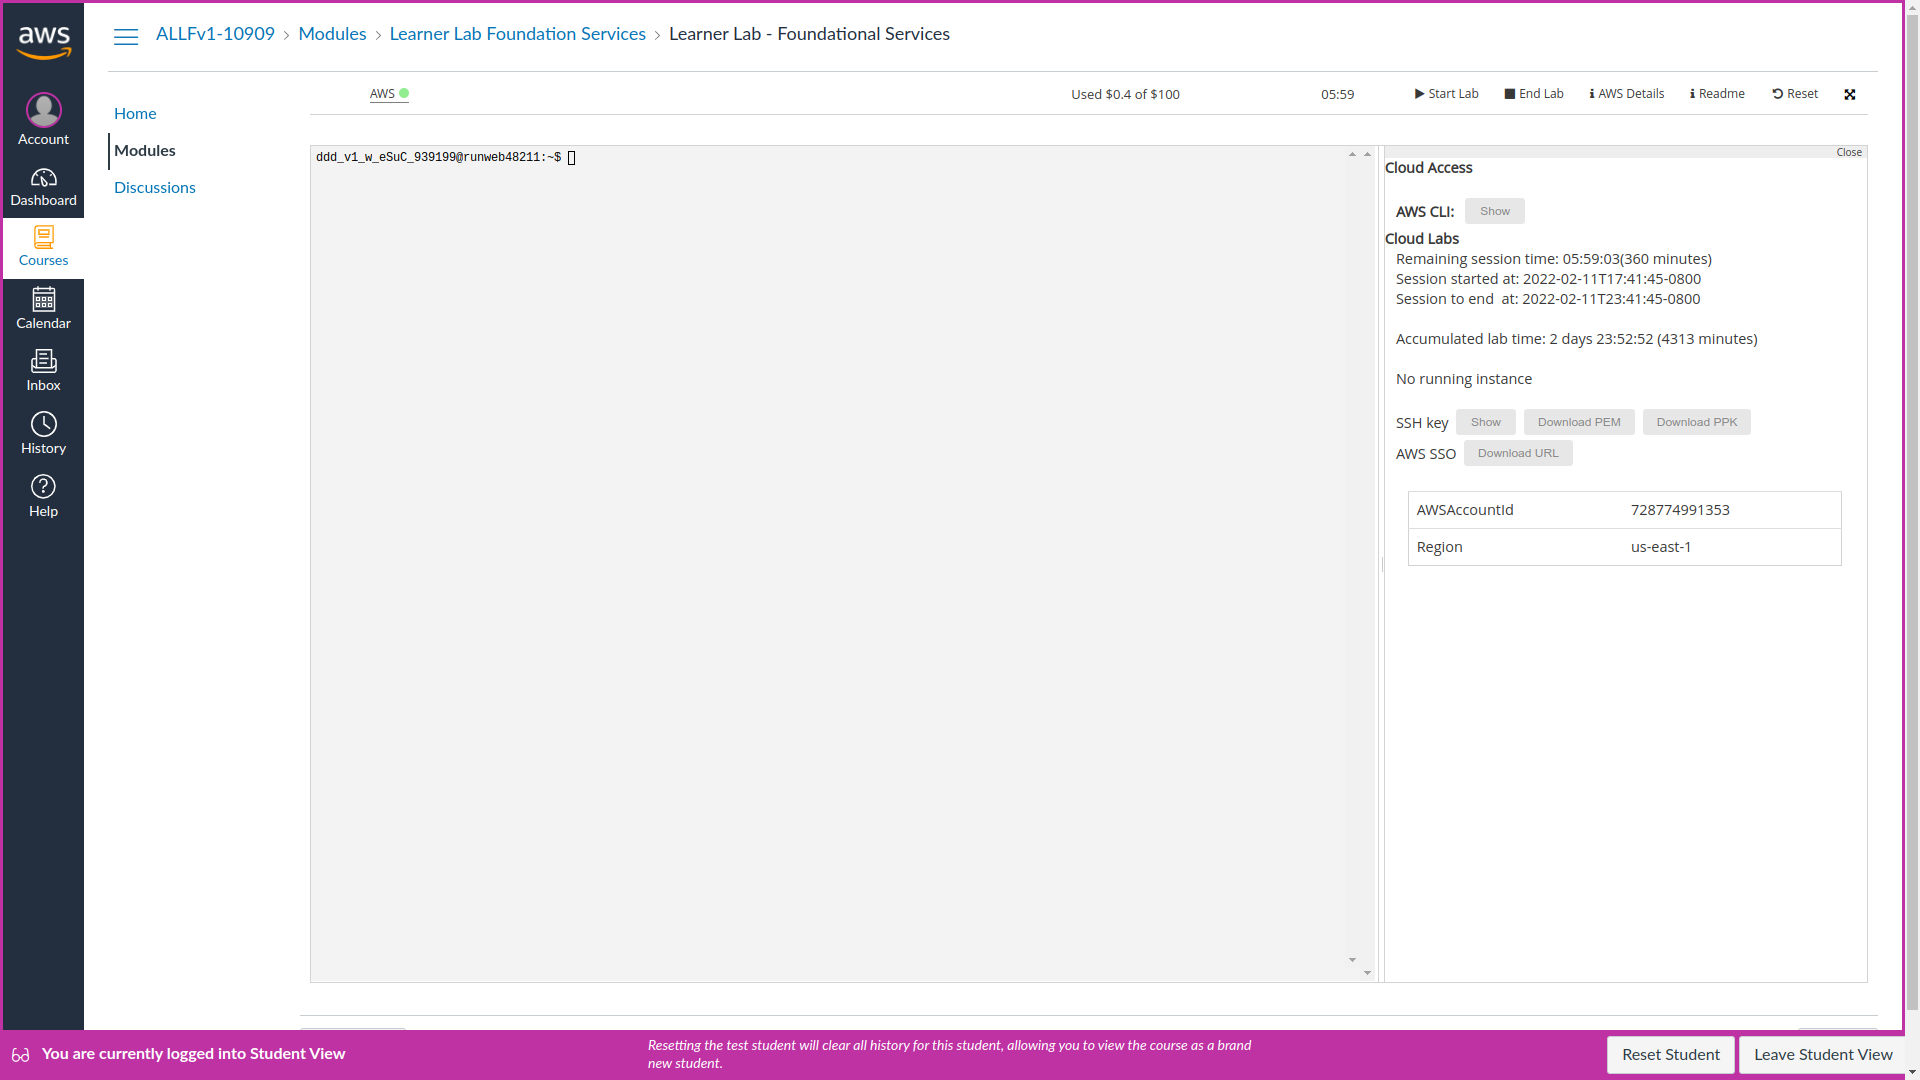
\includegraphics[width=0.7\textwidth]{images/aws-details}

\item Click on the first `Show' button next to `AWS CLI' which will display a text block starting with \texttt{[default]}.
\item Within your repository create a \texttt{credentials} file and copy the contents of the text block into the file.
    \textbf{Do \underline{not} share this file contents --- do \underline{not} commit it}.
\item Create a \texttt{main.tf} file in the your repository with the following contents:
\begin{code}[language=terraform,numbers=none]{main.tf}
terraform {
    required_providers {
        aws = {
            source  = "hashicorp/aws"
            version = "~> 5.0"
        }
    }
}

provider "aws" {
    region = "us-east-1"
    shared_credentials_files = ["./credentials"]
}
\end{code}

\item We need to initialise Terraform which will fetch the required dependencies.
    This is done with the \texttt{terraform init} command.
\bash{terraform init}

This command will create a \texttt{.terraform} directory which stores providers and a provider lock file, \texttt{.terraform.lock.hcl}.

\item To verify that we have setup Terraform correctly, use \texttt{terraform plan}.
\bash{terraform plan}

As we currently have no resources configured, it should find that no changes are required.
Note that this does not ensure our credentials are correctly configured as Terraform has no reason to try authenticating yet.

\end{enumerate}


\section{Deploying a Database in AWS}

\warning{
  This section manually deploys a PostgreSQL RDS instance,
  this is intended as a demonstration by your tutor.
  You should attempt to deploy your infrastructure using Terraform rather than manually.
}

\teacher{
  Instruct the class to observe you making the database and not to follow along.
}

\noindent
To get started let us jump into the lab environment and have a look at AWS RDS which is an AWS managed database service. To get to the RDS service either search for it or browse Services -> Database -> Aurora and RDS, as shown below.

\begin{figure}[H]
\centering
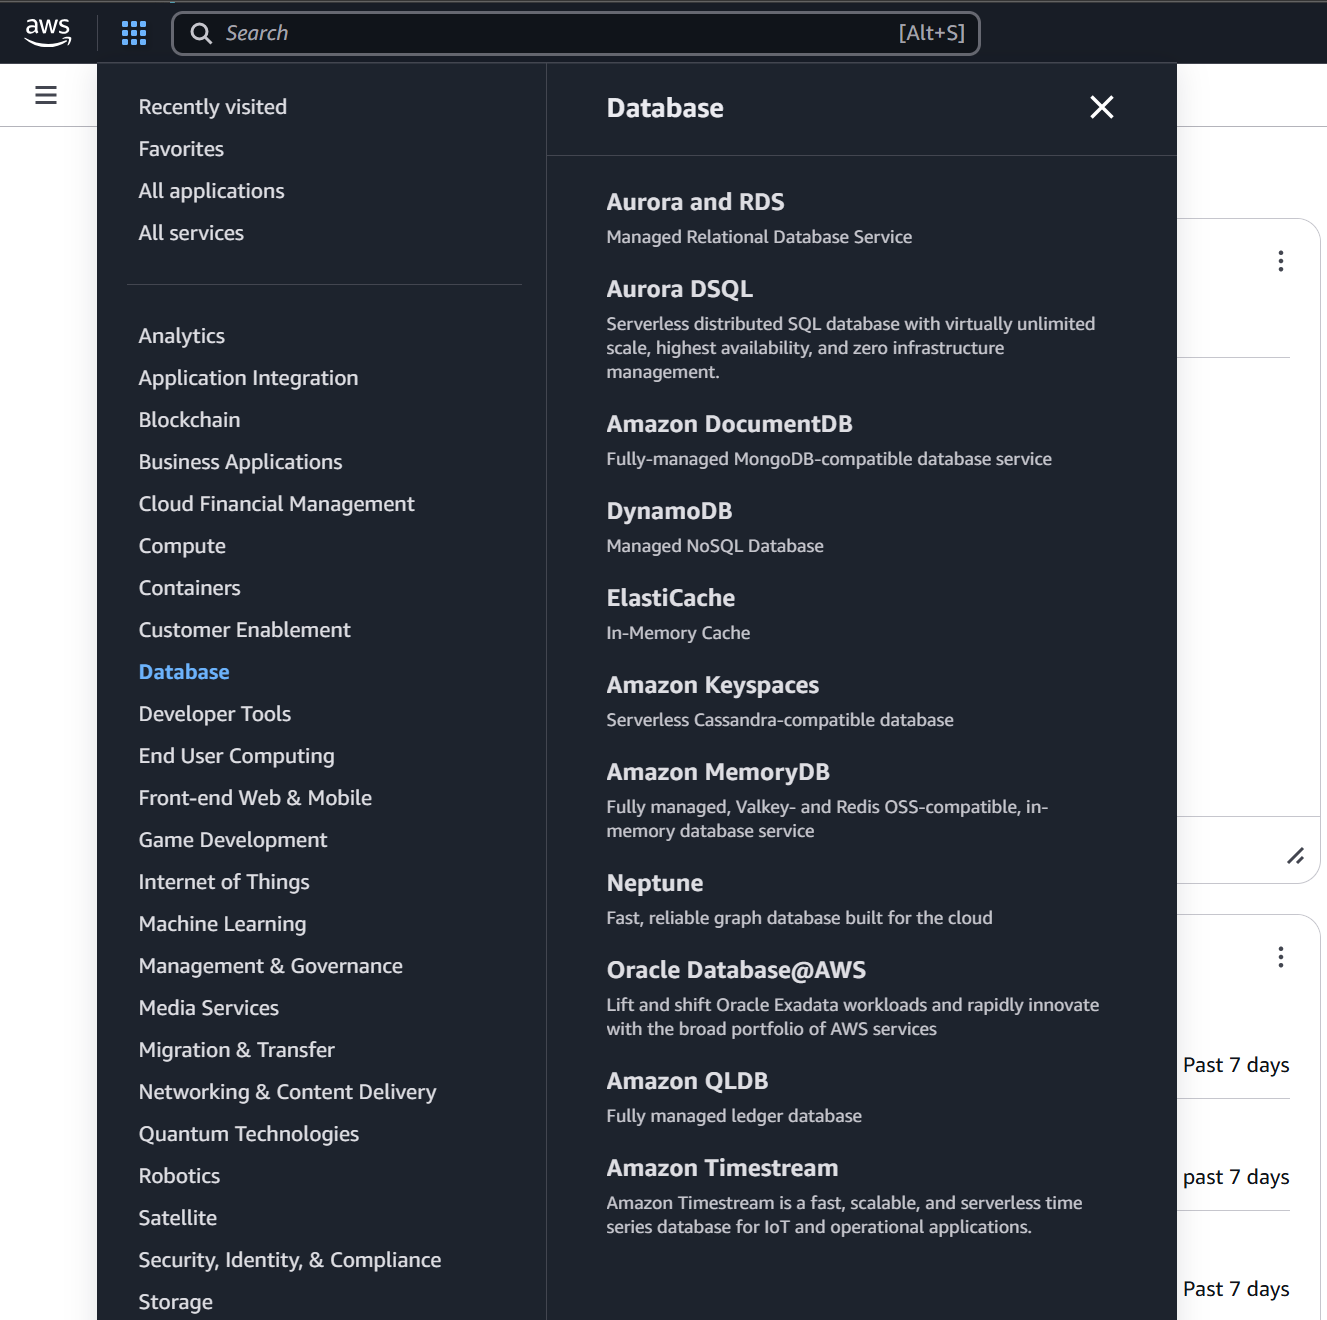
\includegraphics[trim=0 180 0 0,clip,width=0.78\textwidth]{images/aws_1}
\end{figure}

\noindent
Now we are in the management interface for all our RDS instances.
Select ``DB Instances (0/40)'' or click ``Databases'' on the left panel.

\begin{figure}[H]
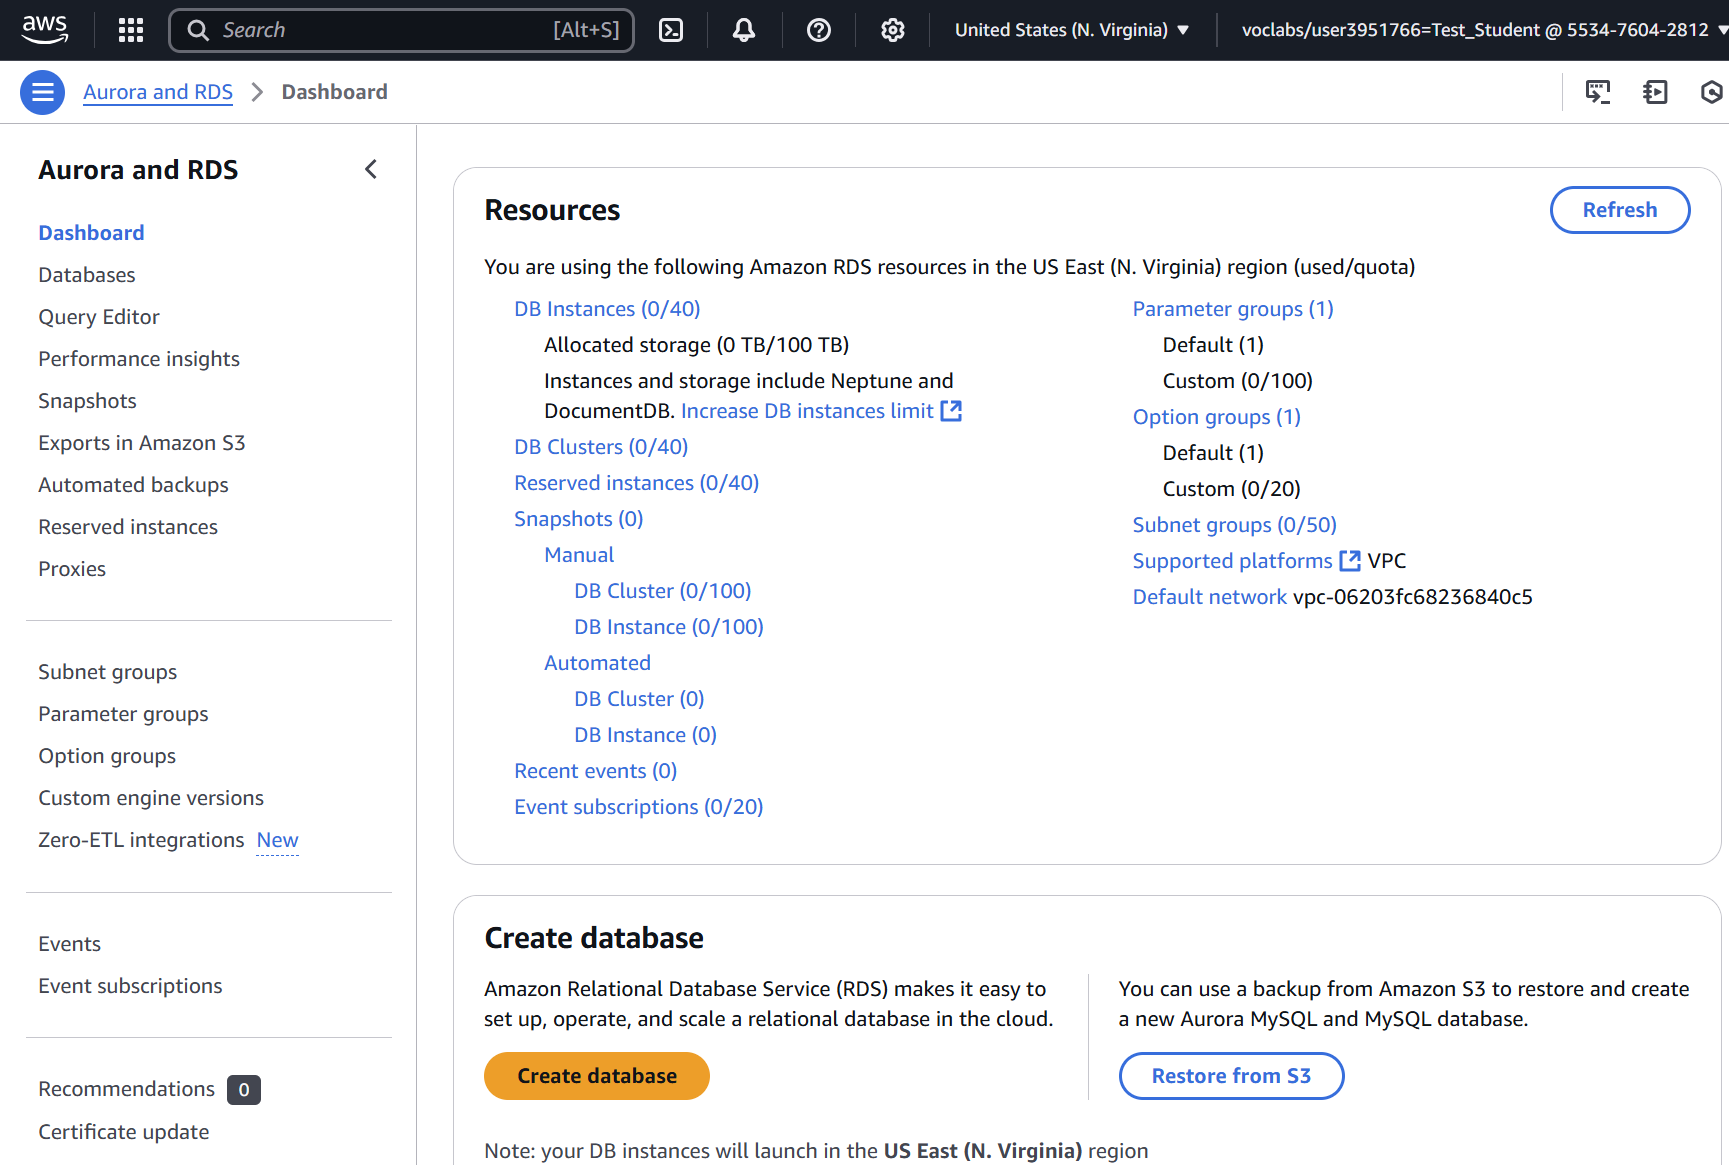
\includegraphics[width=\textwidth]{images/aws_2}
\end{figure}

\noindent
This page should appear familiar as it is very similar to the AWS EC2 instance page.
Let us create a new database by clicking on the ``Create Database'' button.

\begin{figure}[H]
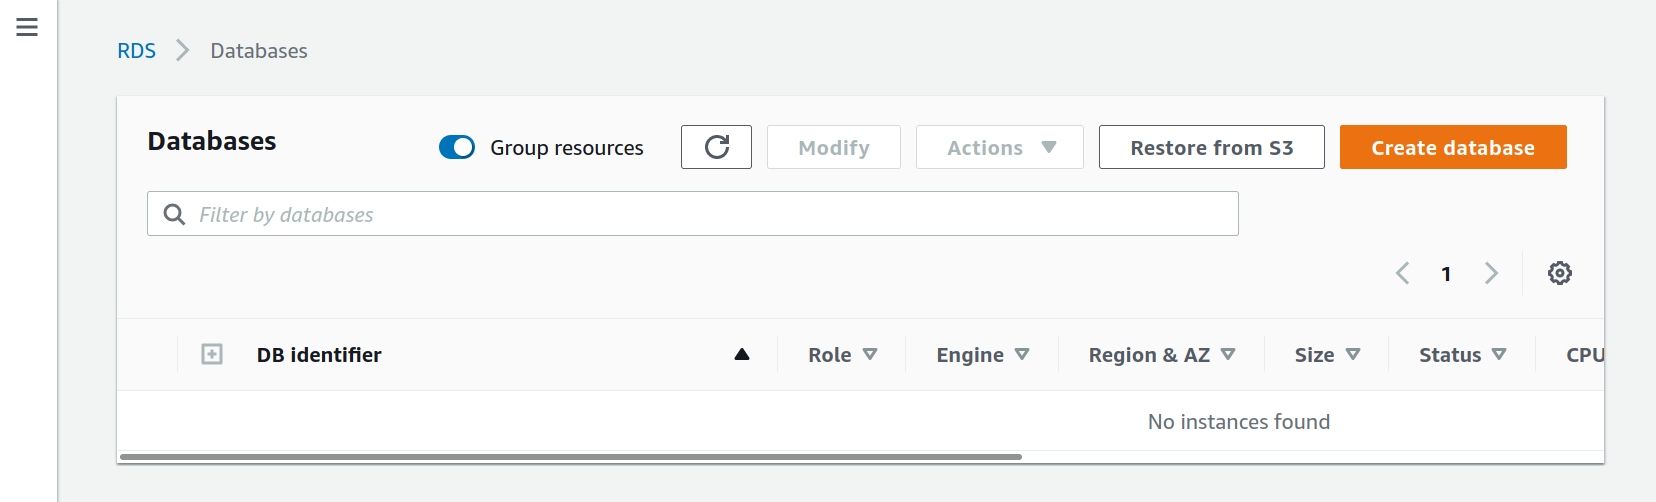
\includegraphics[width=\textwidth]{images/aws_3}
\end{figure}

\warning{
  In the next section we cannot use the Easy Create option as it tries to create an IAM account,
  which is disabled in Learner Labs.
}

\teacher{
  Feel free to talk about the other offerings here, but make sure to flame Oracle and Microsoft SQL Server.
  A good thing to point out is Aurora which is the serverless version of RDS.
}

\newpage
\noindent
We will create a standard database so select standard and PostgreSQL.
We will use version 17, which is a fairly recent release.

\begin{figure}[H]
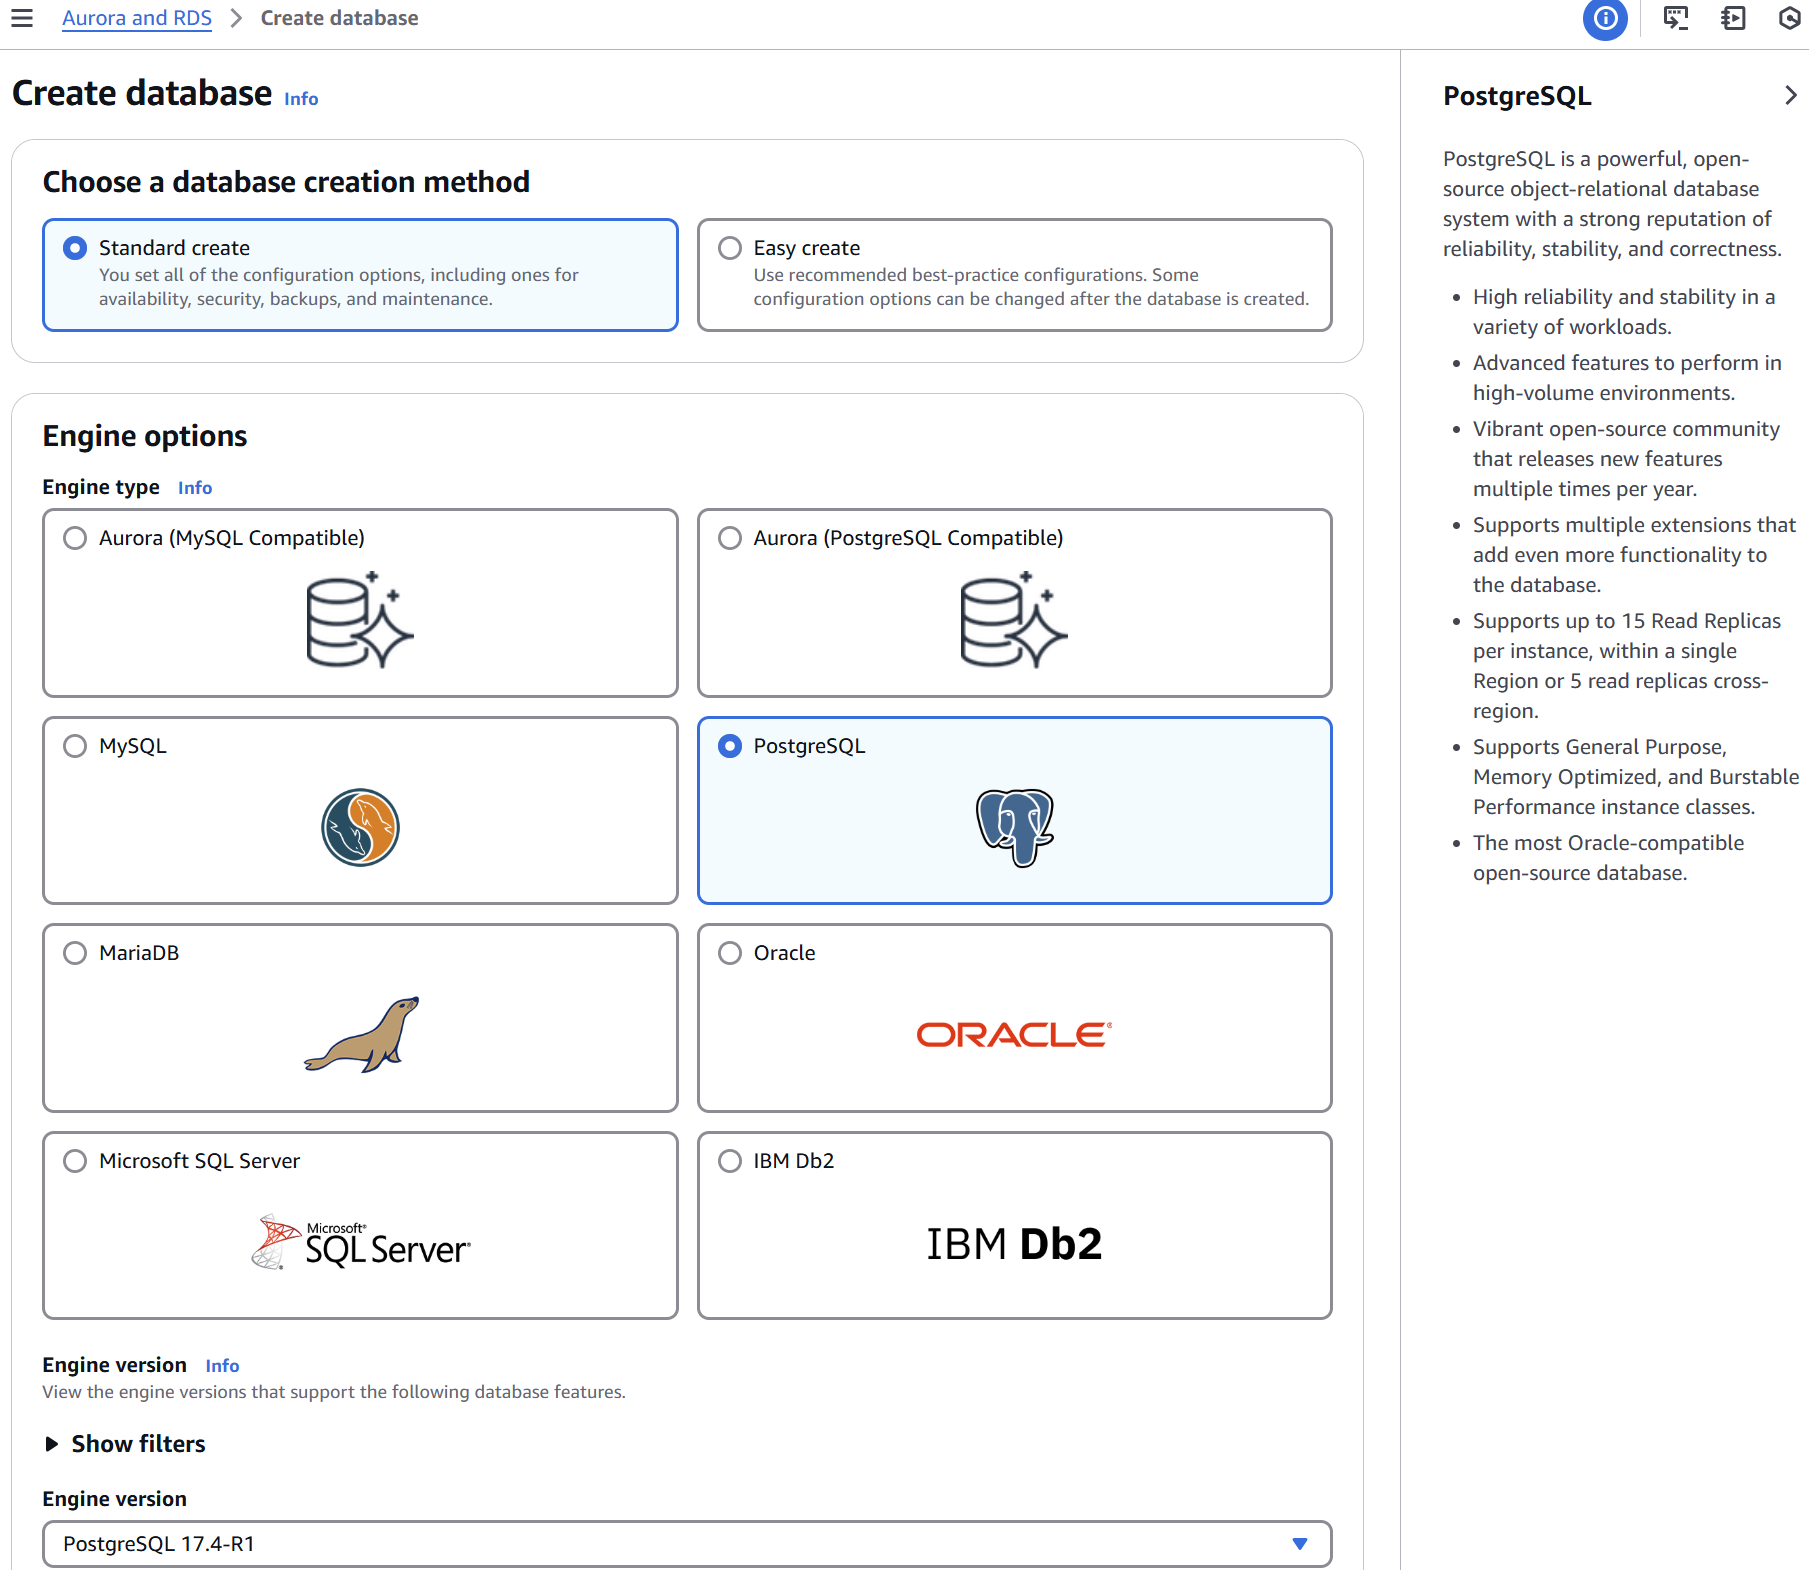
\includegraphics[trim=0 0 220 0,clip,width=\textwidth]{images/db1}
\end{figure}

\newpage
\noindent
For today, we are going to use ``Free Tier'' but in the future,
you may wish to explore the different deployment options.
Please peruse the available options.

\teacher{
  Walk through what Multi-AZ means aka Multiple Availability Zones.
}

\begin{figure}[H]
  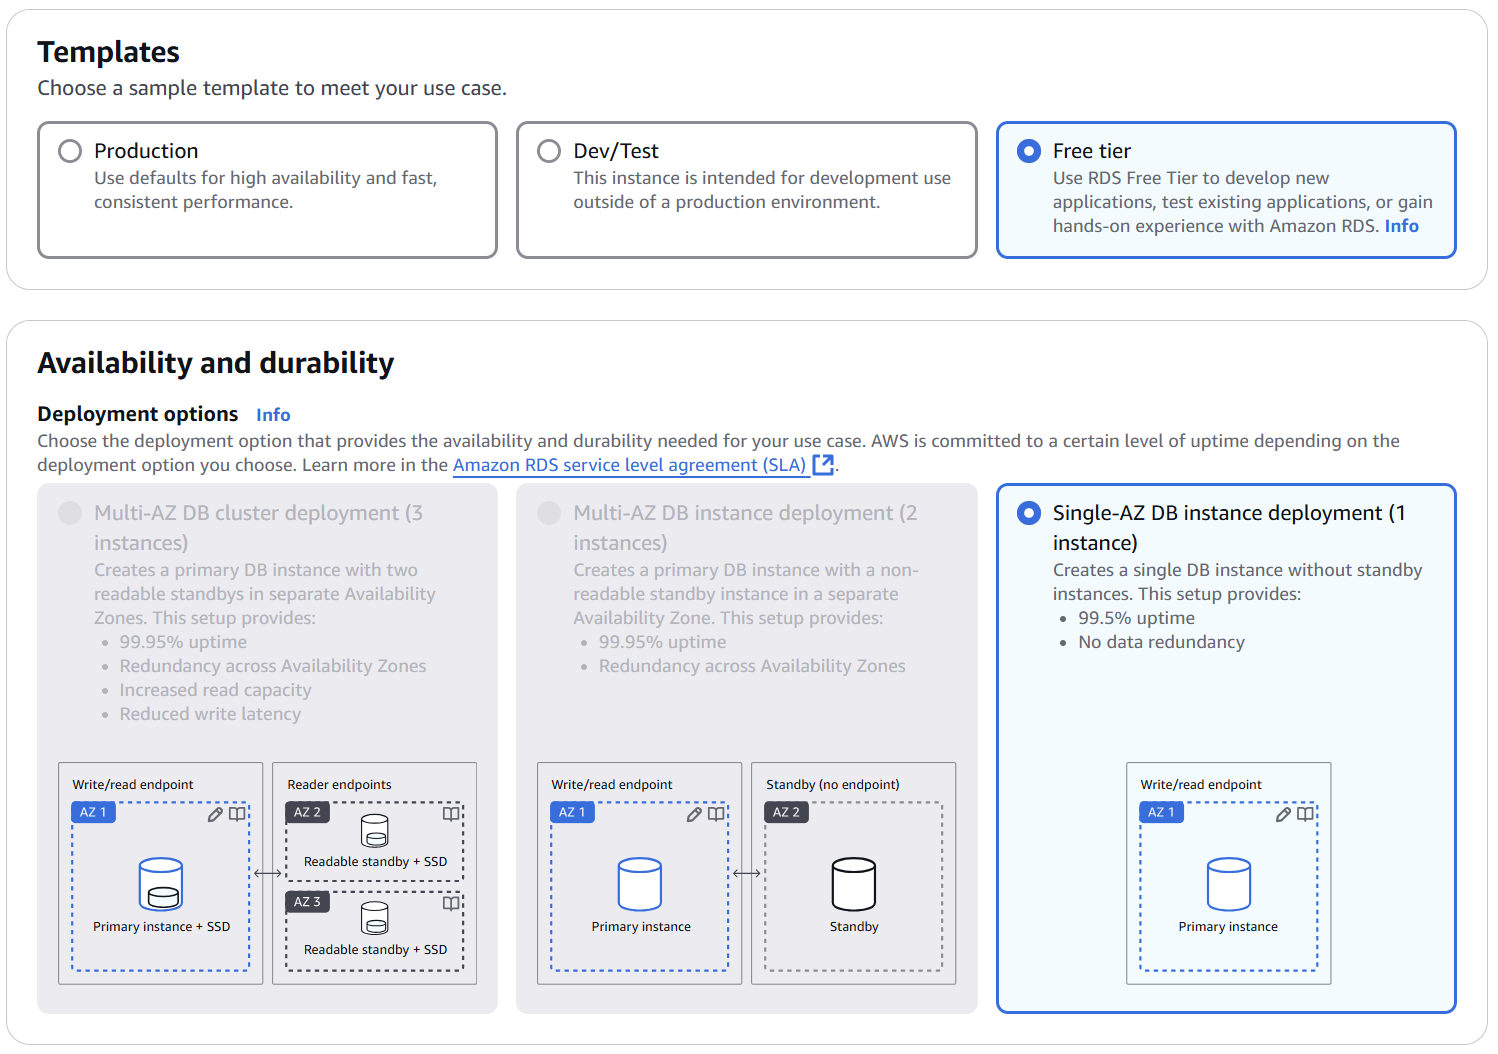
\includegraphics[trim=0 3 0 3,clip,width=\textwidth]{images/db2}
\end{figure}

\newpage
\noindent
Now we need to name our database and create credentials to use when connecting from our application.
Enter memorable credentials as these will be used later.

\begin{figure}[H]
  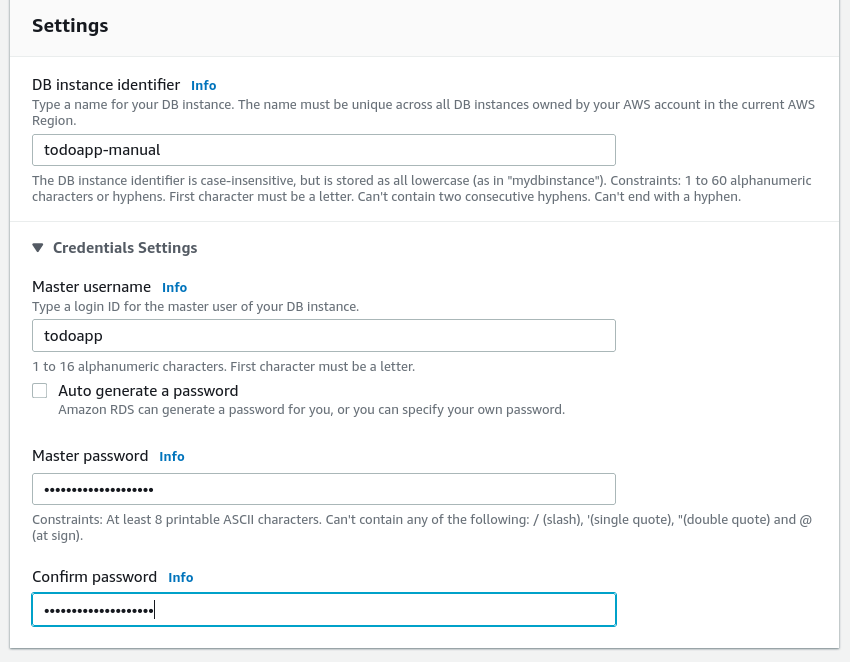
\includegraphics[trim=0 1 0 3,clip,width=\textwidth]{images/db3}
\end{figure}

\noindent
For exploring the process select t3.micro, which should be adequate for our needs.

\teacher{
  May want to mention that burstable is not recommended for consistently used databases.
  Usually DBs are memory focused, so often the selection of memory is more important than the processing capability.
}

\begin{figure}[H]
  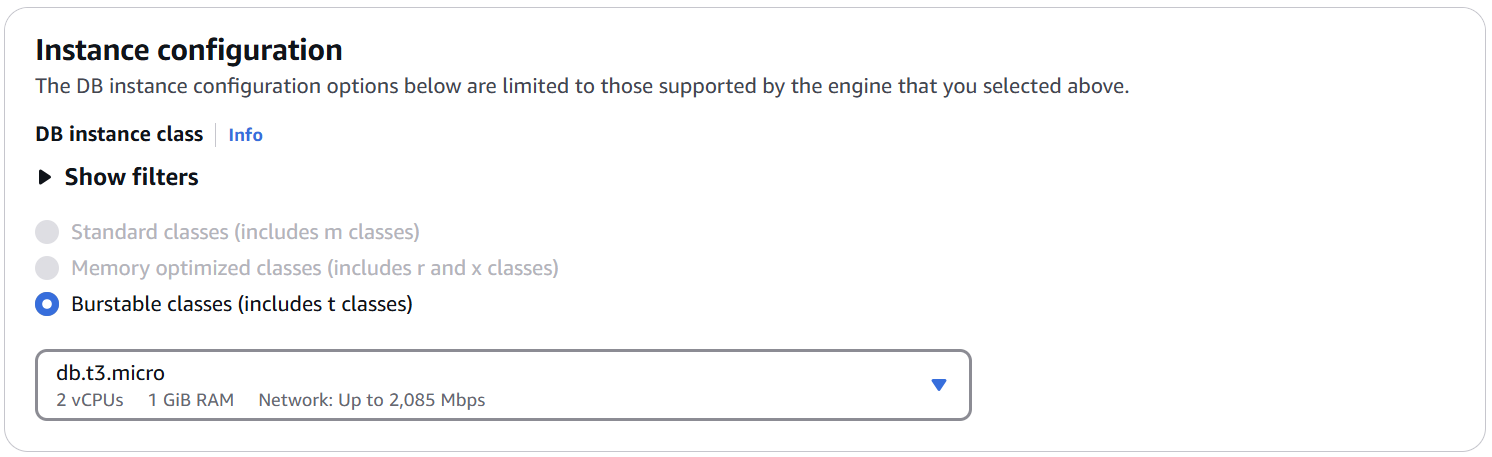
\includegraphics[width=\textwidth]{images/db4}
\end{figure}

\newpage
\noindent
For storage we will leave all the default options.

\begin{figure}[H]
  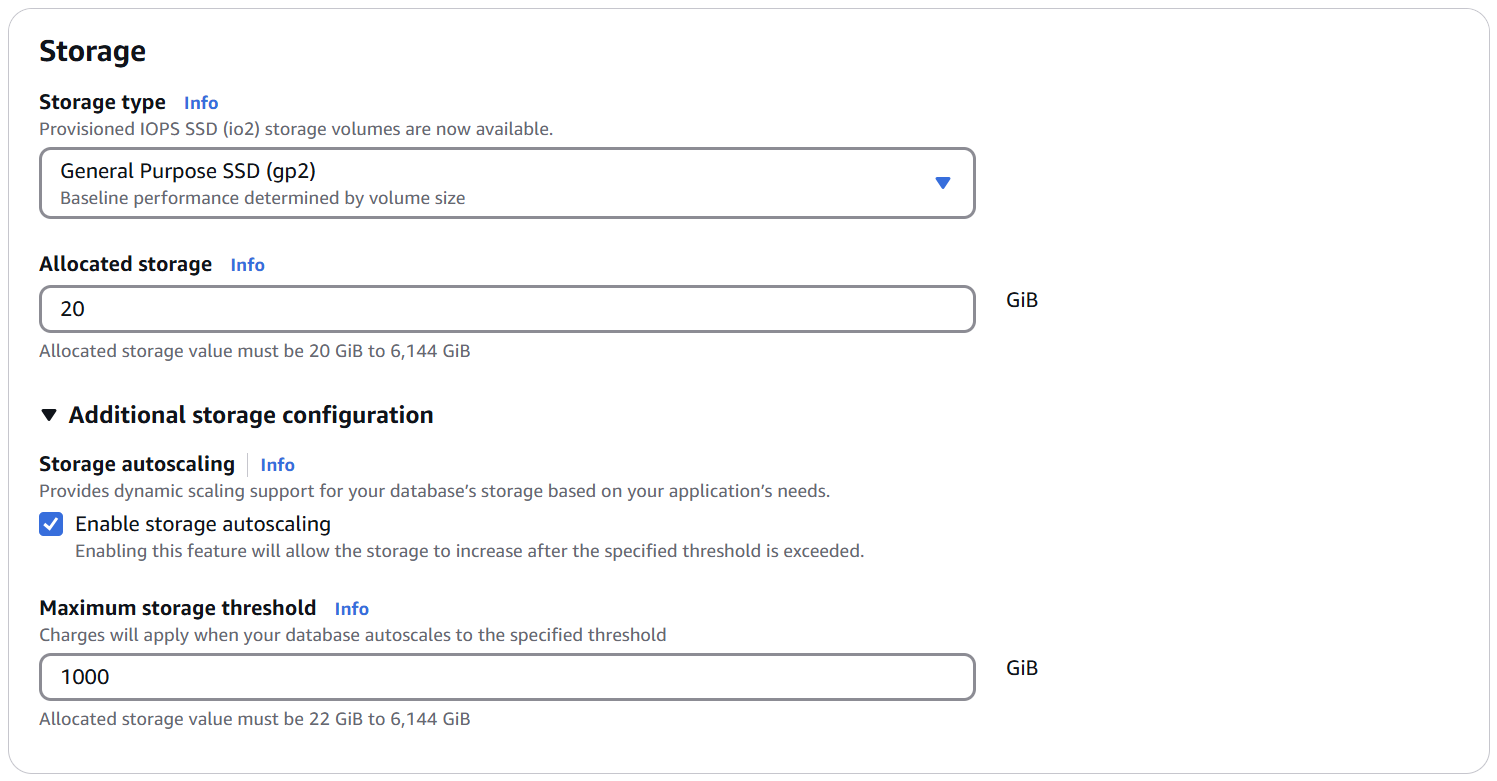
\includegraphics[width=\textwidth]{images/db5}
\end{figure}

\teacher{
  Summarise what each subsection of Connectivity means.
}

\noindent
In connectivity we will leave the \textbf{Compute resource} and \textbf{VPC} with their default values.
We need to make our instance publicly available.
Usually you do \textbf{\textit{not}} want to expose your databases publicly and,
would instead, have a server sitting in-front (e.g. an API, application or web server).
For our learning purposes though we are going to expose it directly just like we did with our EC2 instances earlier in the course.

When selecting public access as yes, we have to create a new Security Group.
Give this Security Group a sensible name.

\begin{figure}[H]
  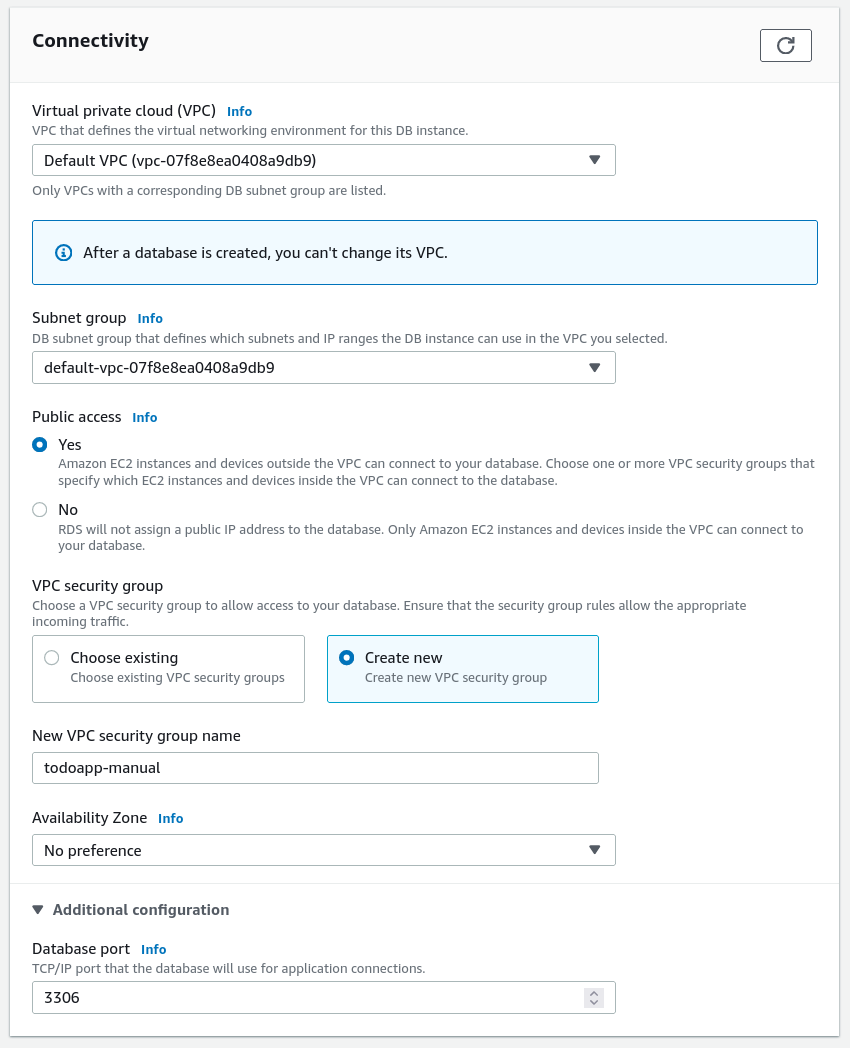
\includegraphics[width=\textwidth]{images/db6}
\end{figure}

\noindent
We will leave the authentication as password based and monitoring with its default values.
We need to expand the ``Additional configuration'' section.
Fill in the ``Initial Database Name'' field as ``todo'',
this will automatically create the database to which our todo application expects to connect.

\teacher{
  The other options here are to do with the parameters used to start the database,
  it is uncommon to have to change these but this is where any settings you would pass in via cli to the db would be set.
}

\begin{figure}[H]
  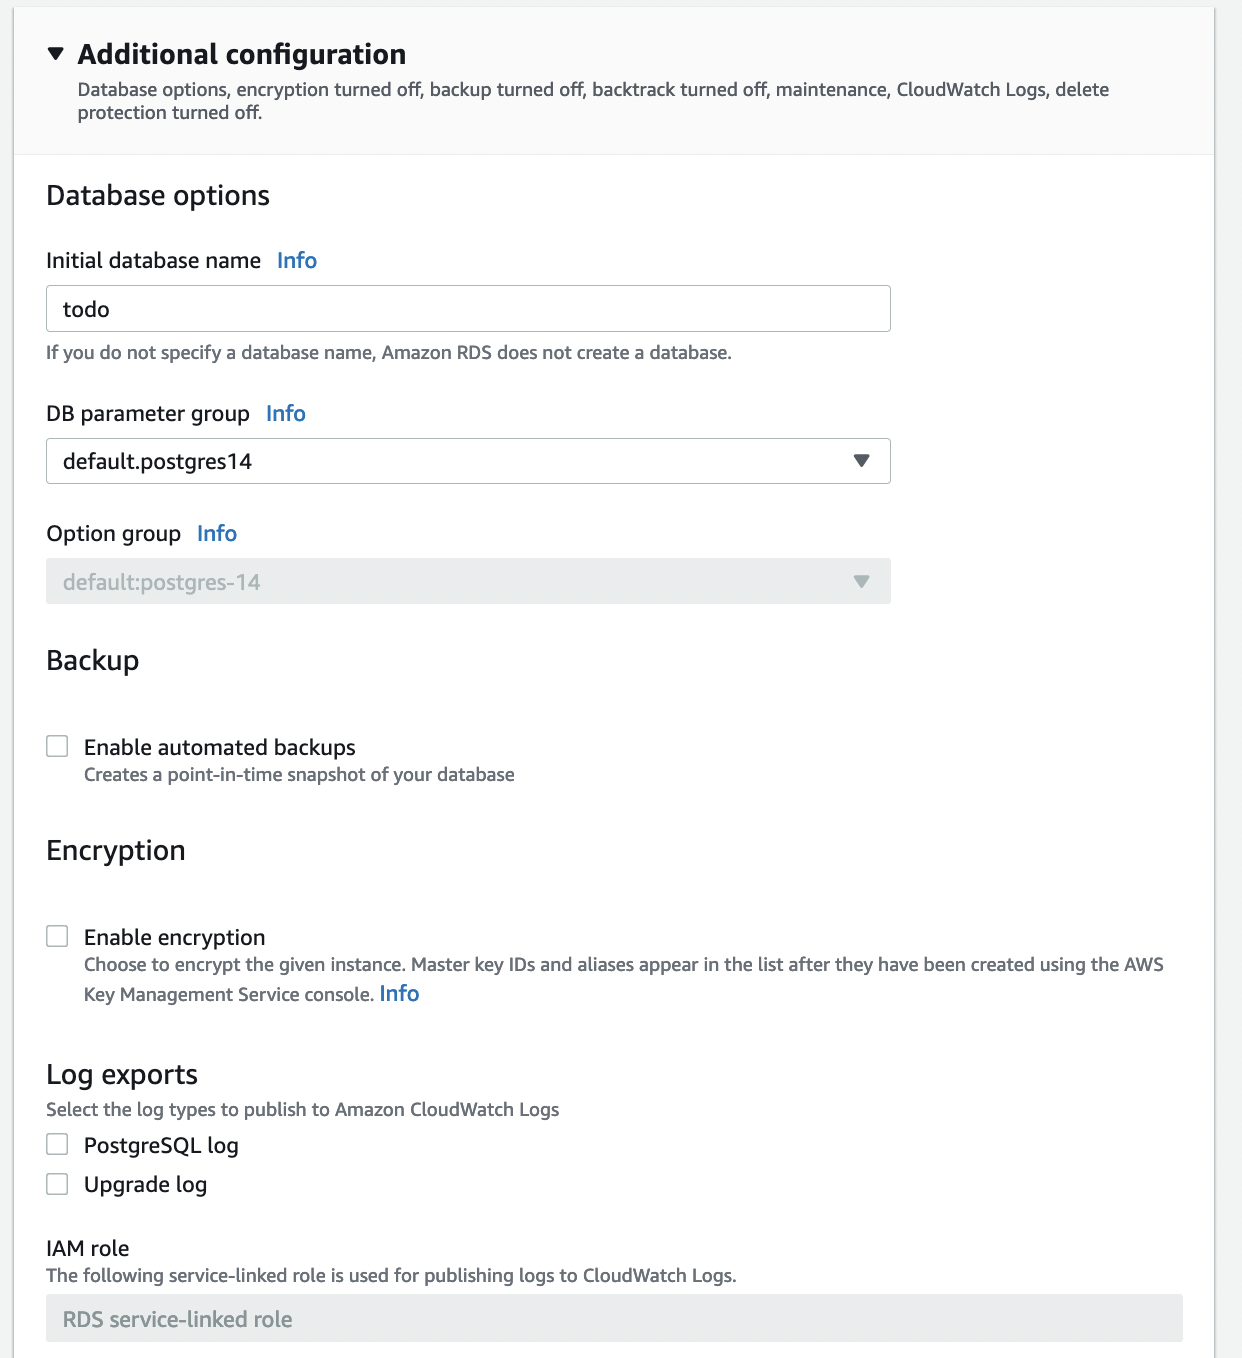
\includegraphics[width=\textwidth]{images/db7}
\end{figure}

\noindent
Now we can click create database, which will take some time.

\begin{figure}[H]
  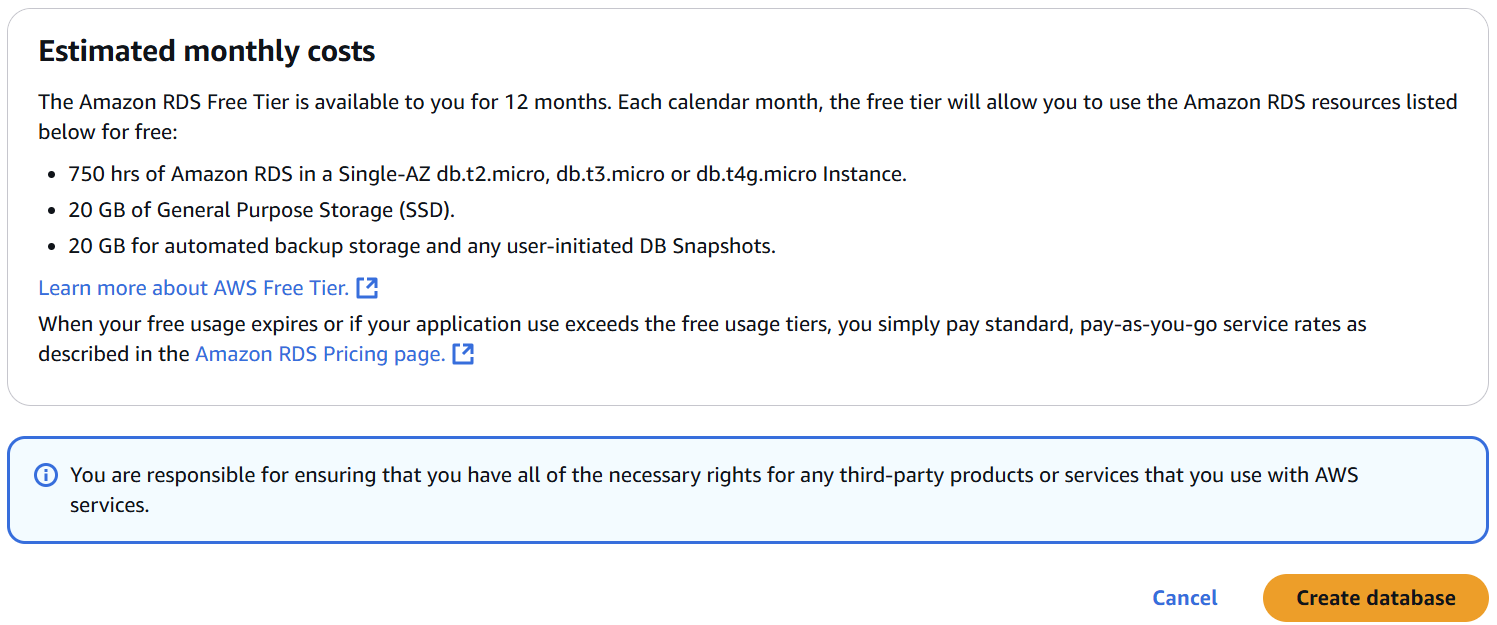
\includegraphics[width=\textwidth]{images/db8}
\end{figure}

\noindent
It may take several minutes to create.
If we had selected to enable automated backups, the database would do an initial backup when it is created.

AWS will suggest add-ons for the newly created database.
The suggested add-ons are useful features for a production environment.
We do not need them for the purposes of this practical.

\begin{figure}[H]
  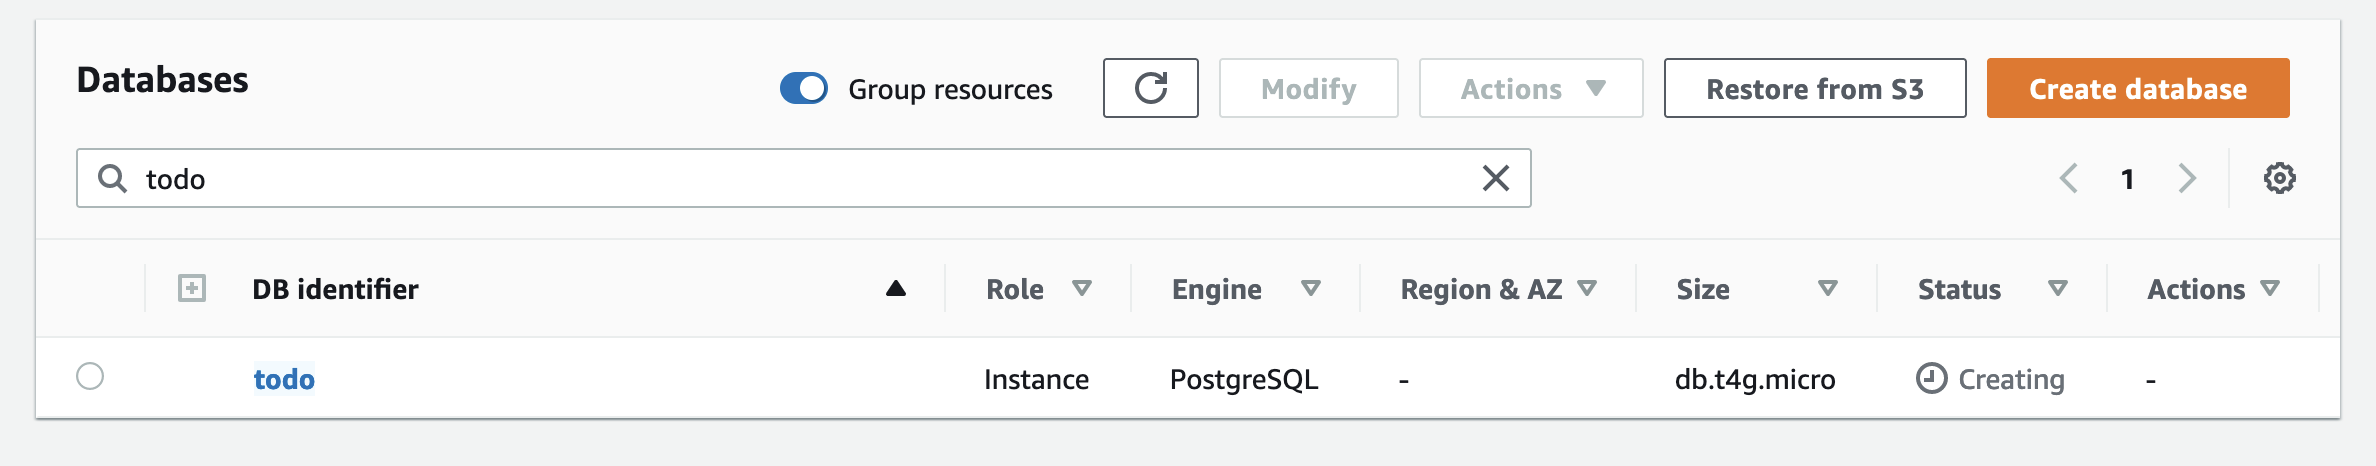
\includegraphics[width=\textwidth]{images/aws_4}
\end{figure}

\noindent
When the database has been created, you can select it to view the configuration and details.
In this menu we also see the endpoint address, which we will need to configure our TaskOverflow application to use.

\begin{figure}[H]
  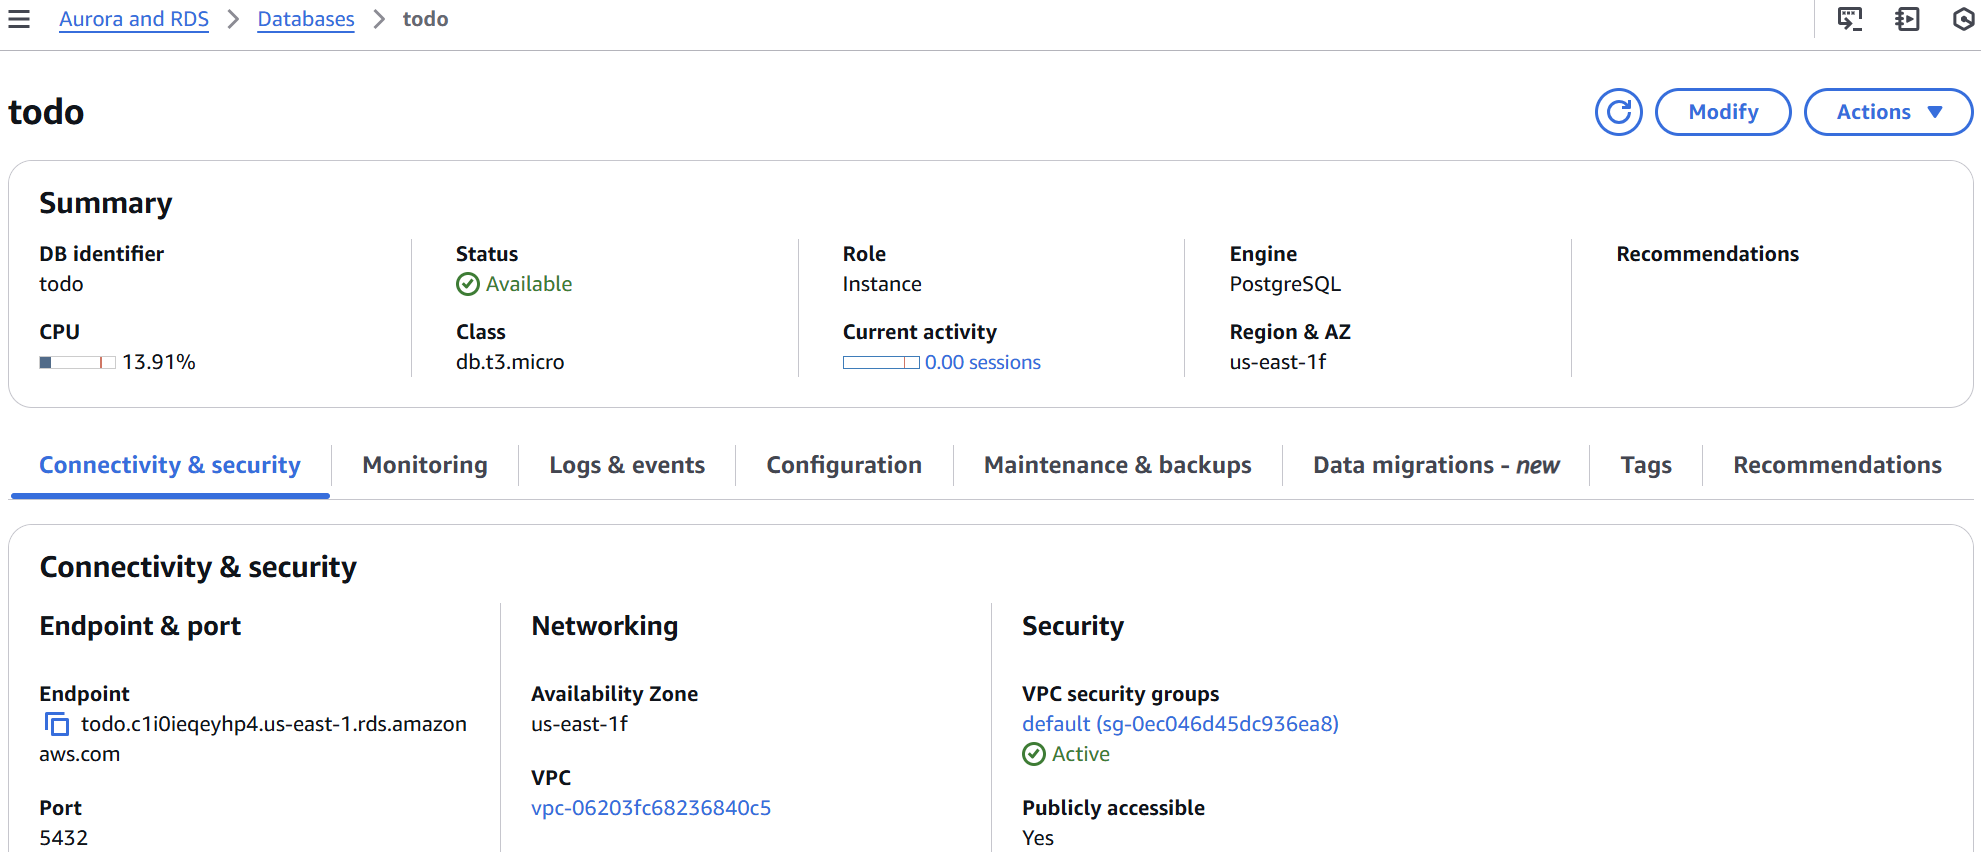
\includegraphics[width=\textwidth]{images/aws_5}
\end{figure}


\section{RDS Database with Terraform}

Now would be a good time to browse the documentation for the RDS database in Terraform.
You will want to get practice at reading and understanding Terraform documentation.

\noindent \url{https://registry.terraform.io/providers/hashicorp/aws/latest/docs/resources/db_instance}

Using our manual configuration, we can come up with a resource with the appropriate parameters as below:

\begin{code}[language=terraform,numbers=none]{main.tf}
locals {
  database_username = "administrator"
  database_password = "foobarbaz"  # This is bad!
}

resource "aws_db_instance" "taskoverflow_database" {
  allocated_storage      = 20
  max_allocated_storage  = 1000
  engine                 = "postgres"
  engine_version         = "17"
  instance_class         = "db.t3.micro"
  db_name                = "todo"
  username               = local.database_username
  password               = local.database_password
  parameter_group_name   = "default.postgres17"
  skip_final_snapshot    = true
  vpc_security_group_ids = [aws_security_group.taskoverflow_database.id]
  publicly_accessible    = true

  tags = {
    Name = "taskoverflow_database"
  }
}
\end{code}

When we created the database using the AWS Console,
we needed an appropriate security group so that we could access the database.
We can create the security group using Terraform as well.

\begin{code}[language=terraform,numbers=none]{main.tf}
resource "aws_security_group" "taskoverflow_database" {
  name        = "taskoverflow_database"
  description = "Allow inbound Postgresql traffic"

  ingress {
    from_port        = 5432
    to_port          = 5432
    protocol         = "tcp"
    cidr_blocks      = ["0.0.0.0/0"]
  }

  egress {
    from_port        = 0
    to_port          = 0
    protocol         = "-1"
    cidr_blocks      = ["0.0.0.0/0"]
    ipv6_cidr_blocks = ["::/0"]
  }

  tags = {
    Name = "taskoverflow_database"
  }
}
\end{code}


\section{Container on AWS}

As we mentioned in the Infrastructure as Code notes \cite{iac-notes},
in this course we will use Docker to configure machines and Terraform to configure infrastructure.
AWS has the ability to deploy Docker containers using a service known as Elastic Container Service (ECS).
We will cover ECS and briefly contrast it to manual deployment via EC2.

For this practical we have made available a Docker container running the TaskOverflow application,
which you can use for your AWS deployment.
This container is available on GitHub under the CSSE6400 organisation:

\url{https://ghcr.io/csse6400/taskoverflow:latest}

This container is very similar to what you have been building in the practicals but contains a simple UI and some extra features for the future practicals.%
\footnote{If you are interested, the source code is available on GitHub \url{https://github.com/csse6400/practical}}

\subsection{Setup}

Of all the different ways that we can deploy our application, we have decided to offload the database to AWS RDS.
This means that we can move all the "state" of our application out of our containerised environment.

To begin, we will reuse the Terraform from above for deploying the RDS database.
Extend the existing local Terraform variables to include the address of the container, so that we have:

\begin{code}[language=terraform,numbers=none]{main.tf}
locals {
  image             = "ghcr.io/csse6400/taskoverflow:latest"
  database_username = "administrator"
  database_password = "foobarbaz" # this is bad
}
\end{code}

This already sets up an RDS instance of Postgres and a security group to allow access to it.
Now we can run \texttt{terraform init} and \texttt{terraform apply} to create our database.
Like when creating the database from the AWS console, this may take several minutes.
Once the database has been created, go to the AWS console and check its status and details.

We have also added a local variable for us to use later.
Variables in Terraform can be populated via two mechanisms,
they can be in a variables block which can be overridden,
or they can be in a locals block which can be used to store values that are used in multiple places.

\subsection{ECS Deployment}
\label{pathb}

\begin{figure}[H]
  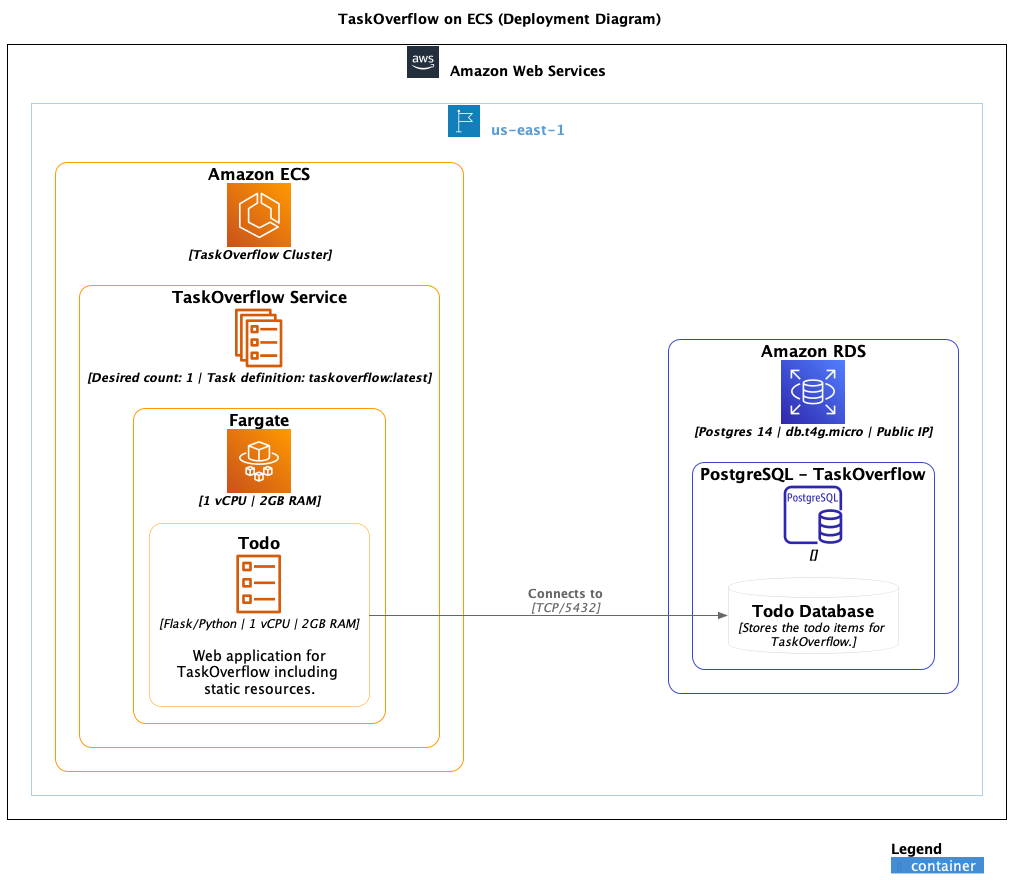
\includegraphics[trim=0 230 0 0,clip,width=\textwidth]{diagrams/ecsdeployment}
\end{figure}

ECS mimics a similar environment as Docker Compose but as an AWS service.

To start off we need to get some information from our current AWS environment so that we can use it later.
Add the code below to fetch the IAM role known as LabRole.
It is a super user in the Learner Lab environments which can do everything you can do through the AWS Console.
We will also fetch the default VPC and the private subnets within that VPC,
 as they are required for the ECS network configuration.

\begin{code}[language=terraform,numbers=none]{}
data "aws_iam_role" "lab" {
    name = "LabRole"
}

data "aws_vpc" "default" {
    default = true
}

data "aws_subnets" "private" {
    filter {
        name   = "vpc-id"
        values = [data.aws_vpc.default.id]
    }
}
\end{code}

In Terraform, the way to retrieve external information is data sources.
These are functionally like resources but they are not created or destroyed,
instead they are populated with attributes from the current state.
See the below for the minor syntactic difference.

\begin{code}[language=terraform,numbers=none,escapechar=!]{}
!\colorbox{yellow}{data}! "aws_iam_role" "lab" {
  ...
}

!\colorbox{yellow}{resource}! "aws_db_instance" "database" {
  ...
}
\end{code}


Now that we have access to the information required,
we can create the ECS cluster to host our application.

The first step is to create the ECS cluster
which is just a logical grouping of any images.
All that is required is a name for the new grouping.

\begin{code}[language=terraform,numbers=none]{main.tf}
resource "aws_ecs_cluster" "taskoverflow" {
    name = "taskoverflow"
}
\end{code}

On its own this cluster is not particularly useful.
We need to create a task definition which is a description of the container that we want to run.
This is where we will define the image that we want to run,
the environment variables,
the port mappings, etc.
This is similar to a server entry in Docker Compose.

\warning{
  The \texttt{<<DEFINITION} line cannot have a trailing space.
  Ensure that one has not been erroneously inserted.
}

\begin{code}[language=terraform,numbers=none]{main.tf}
resource "aws_ecs_task_definition" "taskoverflow" {
    family                   = "taskoverflow"
    network_mode             = "awsvpc"
    requires_compatibilities = ["FARGATE"]
    cpu                      = 1024
    memory                   = 2048
    execution_role_arn       = data.aws_iam_role.lab.arn
  
    container_definitions = <<DEFINITION
  [
    {
      "image": "${local.image}",
      "cpu": 1024,
      "memory": 2048,
      "name": "todo",
      "networkMode": "awsvpc",
      "portMappings": [
        {
          "containerPort": 6400,
          "hostPort": 6400
        }
      ],
      "environment": [
        {
          "name": "SQLALCHEMY_DATABASE_URI",
          "value": "postgresql://${local.database_username}:${local.database_password}@${aws_db_instance.taskoverflow_database.address}:${aws_db_instance.taskoverflow_database.port}/${aws_db_instance.taskoverflow_database.db_name}"
        }
      ],
      "logConfiguration": {
        "logDriver": "awslogs",
        "options": {
          "awslogs-group": "/taskoverflow/todo",
          "awslogs-region": "us-east-1",
          "awslogs-stream-prefix": "ecs",
          "awslogs-create-group": "true"
        }
      }
    }
  ]
  DEFINITION
}
\end{code}

\begin{description}
    \item[family] A family is similar to the name of the task but it is a name that persists through multiple revisions of the task.
    \item[network\_mode] This is the network mode that the container will run in, we want to run on regular AWS VPC infrastructure.
    \item[requires\_compatibilities] This is the type of container that we want to run. This can be fargate, EC2, or external.
    \item[cpu] The amount of CPU units that the container will be allocated. 1024 is equivalen to one vCPU.
    \item[memory] The amount of memory that the container will be allocated, here we've chosen 2GB.
    \item[execution\_role\_arn] The IAM role that the container will run as.
        Importantly, we have re-used the lab role we previously retrieved.
        This gives the instance full admin permission for our lab environment.
    \item[container\_definitions] This is the definition of the container, it should look similar to Docker Compose.
        The only additional feature here is the \texttt{logConfiguration}.
        This configures our container to write logs to AWS CloudWatch, so that we can see if anything has gone wrong.
\end{description}

Now we have a description of our container as a task.
We need a service on which to run the container.
This is functionally similar to an auto-scaling group, as described in the Distributed Systems I lecture \cite{distributed1-slides}.
We specify how many instances of the described container we want and it will provision them.
We also specify which ECS cluster and AWS subnets to run the containers within.

\begin{code}[language=terraform,numbers=none]{main.tf}
resource "aws_ecs_service" "taskoverflow" {
    name            = "taskoverflow"
    cluster         = aws_ecs_cluster.taskoverflow.id
    task_definition = aws_ecs_task_definition.taskoverflow.arn
    desired_count   = 1
    launch_type     = "FARGATE"
  
    network_configuration {
      subnets             = data.aws_subnets.private.ids
      security_groups     = [aws_security_group.taskoverflow.id]
      assign_public_ip    = true
    }
}
\end{code}

In the above we refer to a non-existent security group.
As always, to be able to access our instances over the network we need to add a security group policy to enable it.

\begin{code}[language=terraform,numbers=none]{main.tf}
resource "aws_security_group" "taskoverflow" {
    name = "taskoverflow"
    description = "TaskOverflow Security Group"
  
    ingress {
      from_port = 6400
      to_port = 6400
      protocol = "tcp"
      cidr_blocks = ["0.0.0.0/0"]
    }
  
    ingress {
      from_port = 22
      to_port = 22
      protocol = "tcp"
      cidr_blocks = ["0.0.0.0/0"]
    }
  
    egress {
      from_port = 0
      to_port = 0
      protocol = "-1"
      cidr_blocks = ["0.0.0.0/0"]
    }
}
\end{code}

Finally, if we run the \texttt{terraform apply} command,
it should provision an ECS cluster with a service that will then create one ECS container based on our task description.

Note that we are doing something a bit weird in this deployment.
Normally ECS expects multiple instances of containers,
so it naturally expects a load balancer.
This makes it difficult for us to discover the public IP of our single instance using Terraform.
Instead, you will need to use the AWS Console to find the public IP address.

This is an opportunity for you to explore the ECS interface and find the task, within the service, within the cluster that we have provisioned.

\teacher{
  Demonstrate to students how to navigate to the ECS dashboard to view the cluster and then view the services and tasks.
}

%TODO Update the section above to have multiple instances of the container and add a load balancer.
%TODO Then get the public IP of the load balancer to access the instances.

\subsection{EC2 Deployment}

\aside{
The deployment diagram below is what it would look like, if we deployed our application to an EC2 instance.
As you can see, ECS provides us with features to manage services and tasks for us.
}

\begin{figure}[H]
  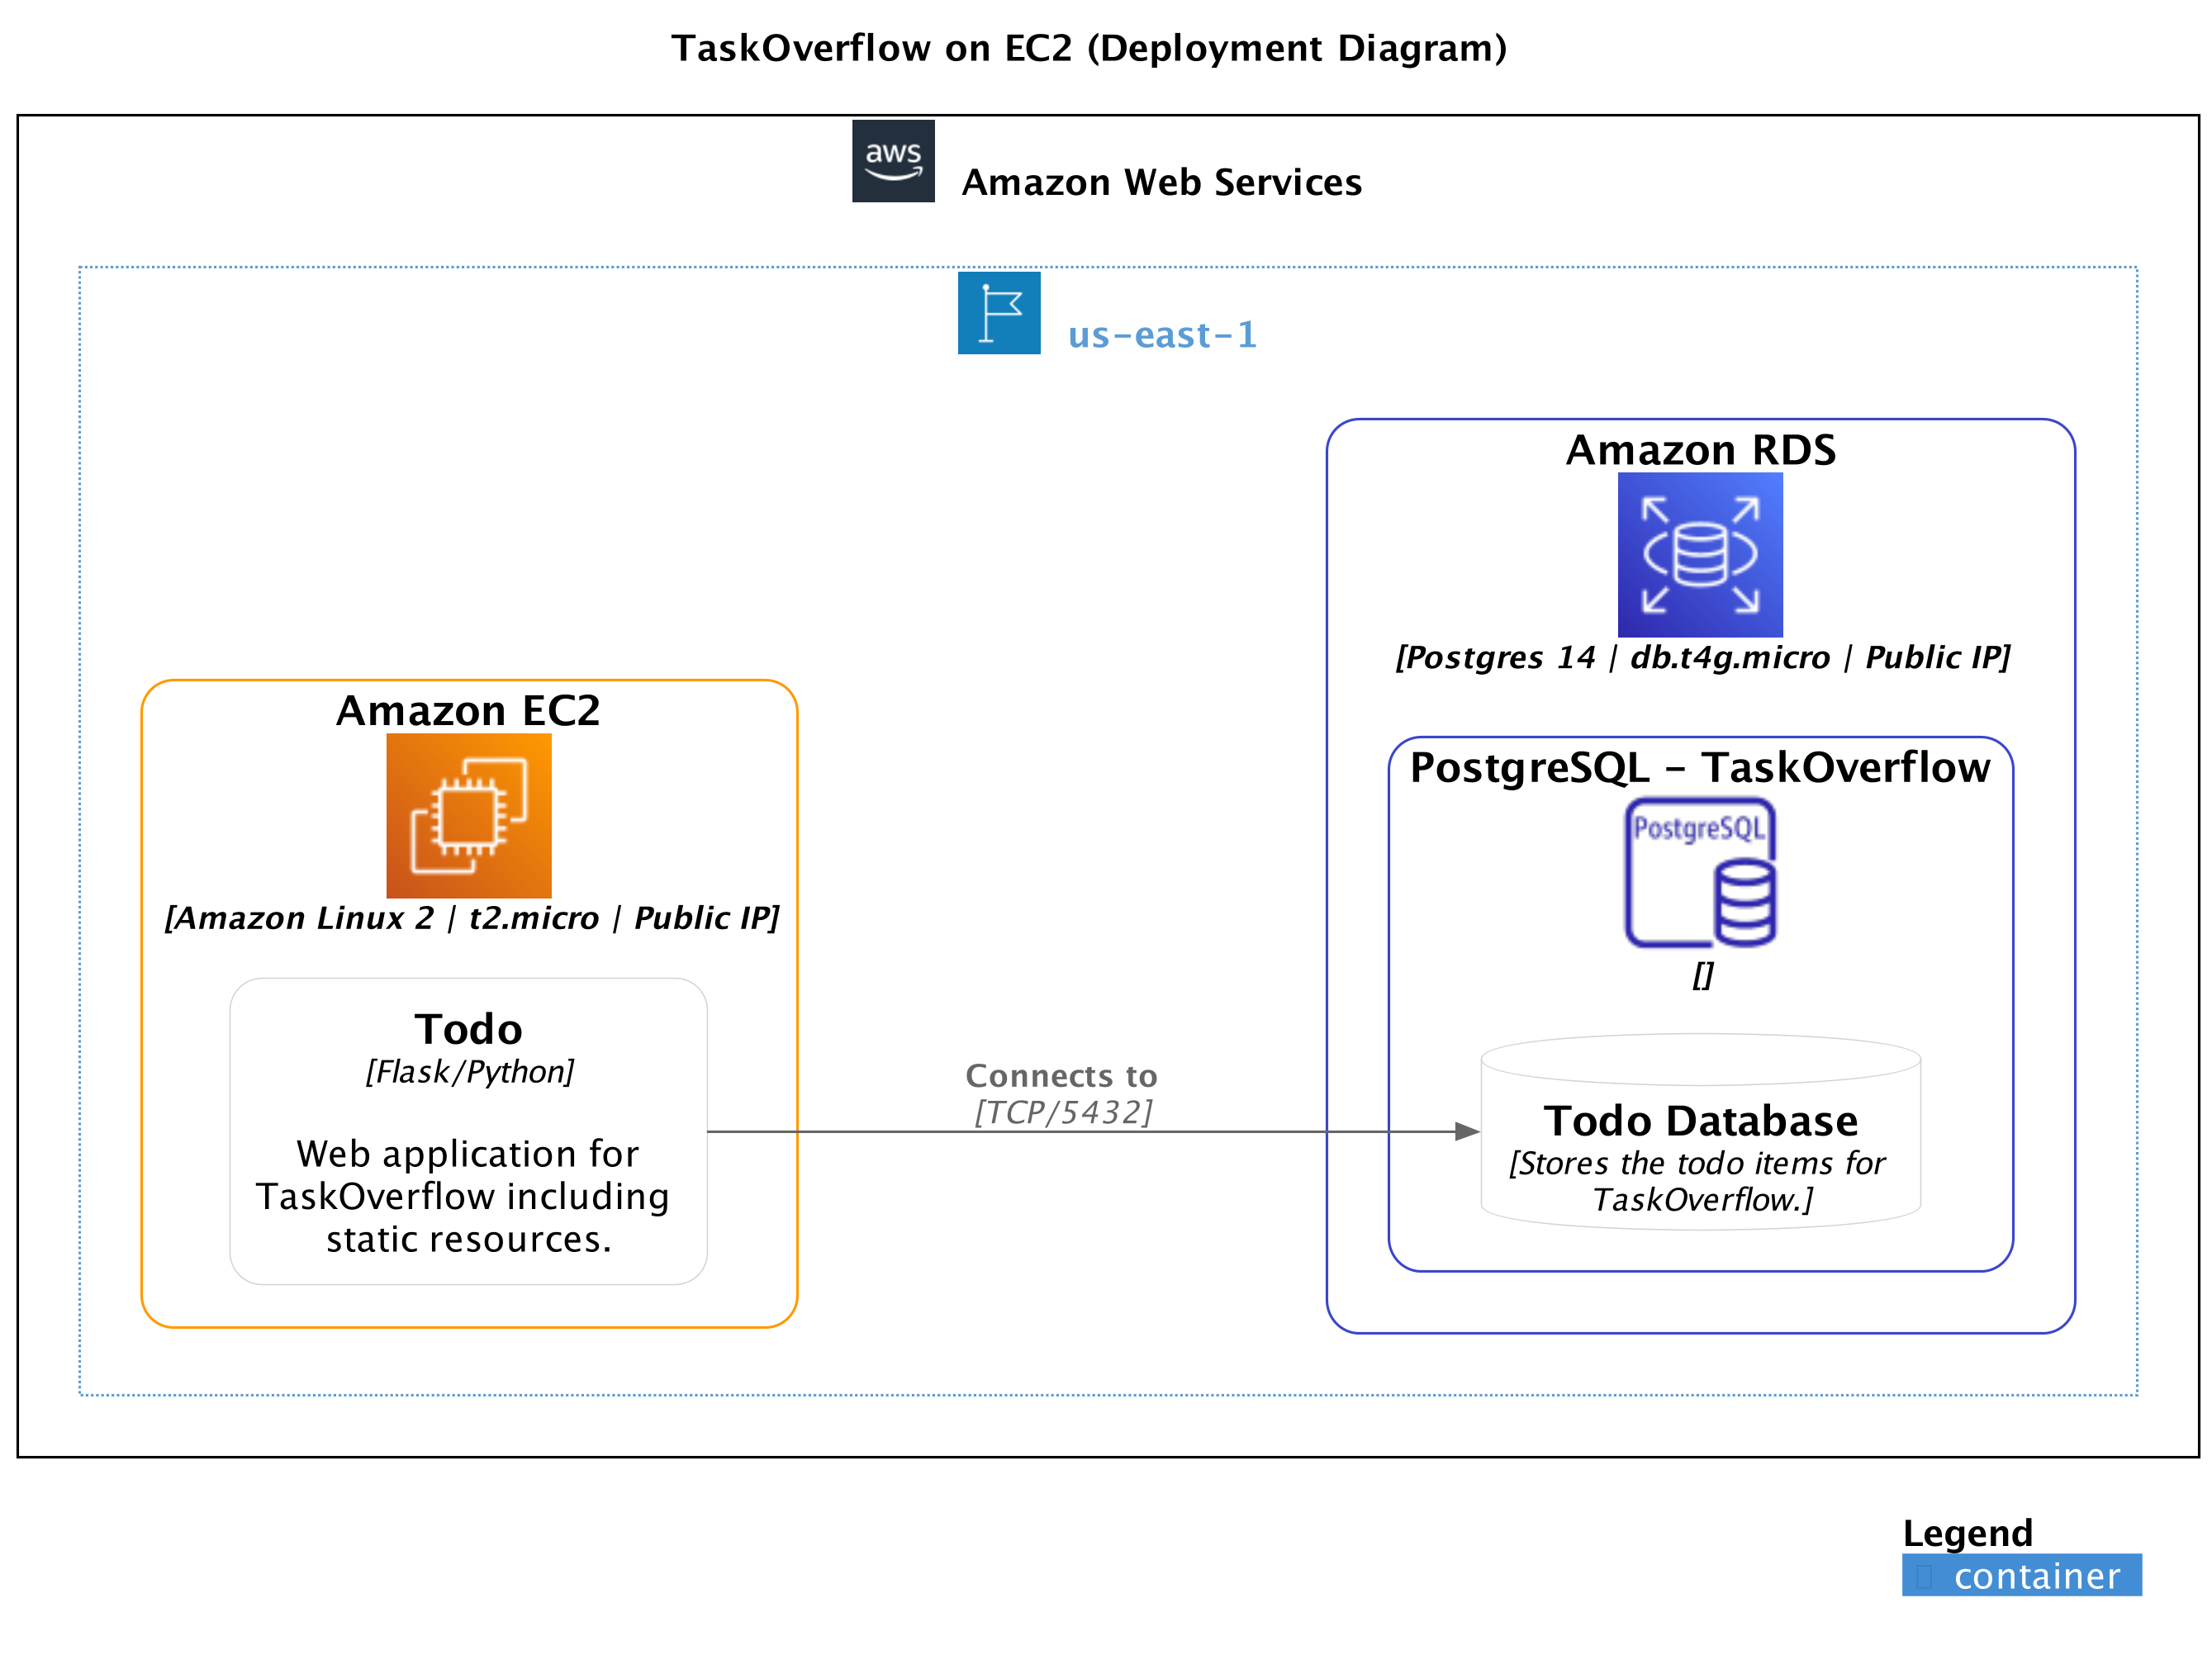
\includegraphics[trim=0 230 0 0,clip,width=\textwidth]{diagrams/ec2deployment}
\end{figure}

\subsection{EKS / K8S}

Amazon Elastic Kubernetes Service (EKS) is a platform to run \link{Kubernetes}{https://kubernetes.io/} (K8S) clusters.
We recommend, when you have time, that you look at Kubernetes as it is widely used in industry.


\section{Hosting TaskOverflow Images}

When we last deployed a container on AWS, we used an existing hosted image.
Now, we will be developing our own image, so we will need a mechanism to host the image.
For this, we will use AWS ECR, Docker, and Terraform.
AWS ECR is the Elastic Container Registry.
It is a container registry like DockerHub or GitHub.
We can use it to host our image.
The steps below use Terraform to

\begin{enumerate}
    \item create an ECR repository for our image,
    \item build our Docker image, and
    \item push our Docker image.
\end{enumerate}

\info{
This is a non-standard process.
As you may have seen in the DevOps tutorial,
we would ordinarily like our code commits to trigger a CI/CD pipeline which builds the images.\\

If you would like, you can use GitHub actions to build and push your container to the GitHub container registry and authenticate when you pull the image.
However, using ECR simplifies the process,
despite the oddities introduced by having a non-persistent ECR repository.
}

\paragraph{Getting Started}

\begin{enumerate}
    \item Using the GitHub Classroom link for this practical provided on Edstem, create a repository to work within.
    \item Install Terraform, if it is not already installed, as it will be required again this week and in later weeks.
    \item Start your Learner Lab and copy the AWS Learner Lab credentials into a credentials file in the root of the repository.
\end{enumerate}

\paragraph{What's New}
We are starting again with our todo application from roughly where we left off in the week 3 practical.
We have added a new directory \texttt{todo/app} that has the static HTML files for the TaskOverflow website and added a route to serve these files.
We have also created a production version of the server that uses gunicorn,
the \texttt{bin} directory is used by this image.
Our original Docker image is now in \texttt{Dockerfile.dev}.\\


We will setup our initial Terraform configuration.
Note that now we introduce a new required provider.
This provider is for Docker.

\begin{code}[language=terraform,numbers=none]{main.tf}
terraform {
   required_providers {
      aws = {
         source = "hashicorp/aws"
         version = "~> 5.0"
      }
      docker = {
         source  = "kreuzwerker/docker"
         version = "3.0.2"
      }
   }
}

provider "aws" {
   region = "us-east-1"
   shared_credentials_files = ["./credentials"]
}
\end{code}

As with our AWS provider,
when we initially configure the provider,
we want to authenticate so that we can later push to our registry using the Docker provider.
We will use the \texttt{aws\_ecr\_authorization\_token} data block to get appropriate ECR credentials for Docker.

\begin{code}[language=terraform,numbers=none]{main.tf}
data "aws_ecr_authorization_token" "ecr_token" {}

provider "docker" {
  registry_auth {
    address  = data.aws_ecr_authorization_token.ecr_token.proxy_endpoint
    username = data.aws_ecr_authorization_token.ecr_token.user_name
    password = data.aws_ecr_authorization_token.ecr_token.password
  }
}
\end{code}

We need to use Terraform to create an ECR repository to push to.

\begin{code}[language=terraform,numbers=none]{main.tf}
resource "aws_ecr_repository" "taskoverflow" {
  name = "taskoverflow"
}
\end{code}

\noindent
The URL for containers in the ECR follow the format below:

\url{{ACCOUNT_ID}.dkr.ecr.{REGION}.amazonaws.com/{REPOSITORY_NAME}}

Remember --- to push to a container registry
we need a local container whose tag matches the remote URL.
We could then create and push the container locally with:

\begin{code}[language=bash,numbers=none]{}
docker build -t {ACCOUNT_ID}.dkr.ecr.{REGION}.amazonaws.com/{REPOSITORY_NAME} .
docker push {ACCOUNT_ID}.dkr.ecr.{REGION}.amazonaws.com/{REPOSITORY_NAME} 
\end{code}

However, it would be easier if we could build and push this container from within Terraform.
We can use the Docker provider for this.

\begin{code}[language=terraform,numbers=none]{image.tf}
resource "docker_image" "taskoverflow" {
  name         = "${aws_ecr_repository.taskoverflow.repository_url}:latest"
  build {
    context = "."
  }
}

resource "docker_registry_image" "taskoverflow" {
  name          = docker_image.taskoverflow.name
}
\end{code}

Notice that we are able to utilise the output of the ECR repository as the URL which resolves to the correct URL for the image.

If you execute \texttt{terraform plan}, it will probably report an inconsistent dependency.
This is because we have added a new provider and its dependency needs to be added to the lock file.
Execute \texttt{terraform init -upgrade} to do this.

You can now \texttt{terraform apply} to push the container to the registry.
Note that the Docker Engine / Daemon must be running so Terraform can talk to it.

\bibliographystyle{ieeetr}
\bibliography{books,ours}

\end{document}
